\documentclass{report}
\usepackage{graphicx}
\usepackage{amsmath}
\usepackage{rotating}
\usepackage{appendix}
\usepackage{mathtools}
\setlength{\parskip}{1em}
\renewcommand{\abstractname}{Summary}
\usepackage{nomencl}
\usepackage{multirow}
\usepackage{placeins}
\makenomenclature

\begin{document}
\begin{titlepage}
	\centering
	
\includegraphics[width=0.25\textwidth]{graphics/logo}\par\vspace{1cm}
	{\scshape\LARGE University of Bath \par}
	\vspace{1cm}
	{\scshape\Large FINAL YEAR Meng PROJECT REPORT\par}
	\vspace{1cm}
	{\huge\bfseries Wave energy converter power increase through active control: Fixed Gains\par}
	\vspace{2cm}
	{\Large\itshape Carl Selig\par}

	\vfill
	
	supervised by\par
	Dr.~Andrew \textsc{Hillis}\par
	assessed by\par
	Dr.~Joseph \textsc{Flynn}

	\vfill
	
\tiny{I certify that I have read and understood the entry in the Student Handbook for the
Department of Mechanical Engineering on Cheating and Plagiarism and that all
material in this assignment is my own work, except where I have indicated with
appropriate references. Signed: ...........}

% Bottom of the page
	{\large \today\par}
\end{titlepage}

\begin{abstract}
Lorem ipsum
\end{abstract}
\section*{Acknowledgements}
I would like to thank Dr. Andrew Hillis for going above and beyond the role of supervisor. I also wish to thank my family, my friends, and especially my therapist: Laura Keyte.
\tableofcontents
\listoffigures
\listoftables

\mbox{}

\nomenclature{$WEC$}{Wave Energy Converter}
\nomenclature{$IMC$}{Internal Model Control}
\nomenclature{$DOF$}{Degree(s) of Freedom}
\nomenclature{$SISO$}{Single Input Single Output}
\nomenclature{$MIMO$}{Multiple Input Multiple Output}
\nomenclature{$Plant$}{The physical system which is being controlled}
\nomenclature{$MATLAB$}{Matrix Laboratory. A programming language and development environment specialised for the manipulation of matrices.}
\nomenclature{$Simulink$}{A graphical programming environment based on MATLAB. Users manipulate dynamic systems by placing and connecting blocks.}

\printnomenclature

\chapter{Introduction}
This report seeks to present the results of the research project conducted by the Author as well as the means to reproduce them. The project is part of a larger research effort to increase the power generation of Wave Energy Converters (WECs) through control system design. It is hoped that improved power generation will increase the commercial viability of the field. Wave power is already considered a viable energy source for the UK \cite{carbonTrust} but has not seen significant implementation at the time of writing \cite{europeanMarineEnergyCenter}.

Wave power refers to a group of technologies that harvest energy from sea waves. It is distinct from Tidal power. Wave power is relevant as a renewable energy source that has advantages over other sources such as solar and wind. Most notably, it constantly produces a base amount of power; can be used along most coastlines; and has a low initial expenditure. \cite{carbonTrust}

The WEC examined in this project is modelled after the Wave Sub device developed by Marine Power Systems\cite{waveSub}. \ref{fig:waveSub} shows a published graphic\cite{waveSub} of this device against the modelled WEC. It was chosen as a generic example of a multi-DOF WEC. The Carbon Trust describes multi-DOF WECs as being of particular interest to UK energy infrastructure due to their increased potential for energy capture over single DOF WECs \cite{carbonTrust}.



\begin{figure}
\centering
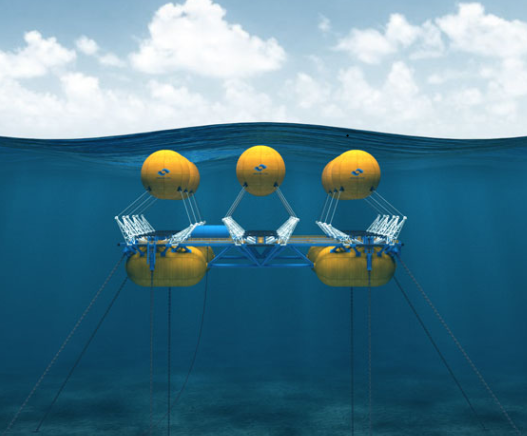
\includegraphics[height=0.4\textwidth]{graphics/waveSub}
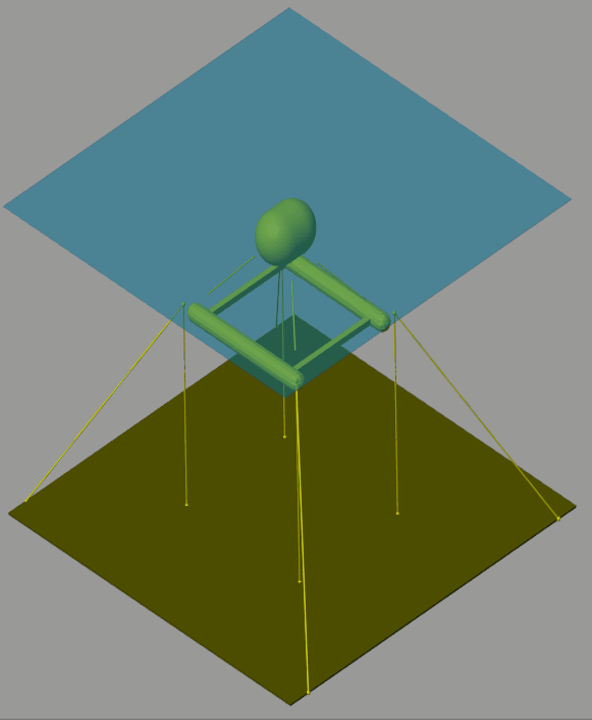
\includegraphics[height=0.4\textwidth]{graphics/wecSimFloat}
\label{fig:waveSub}
\caption{A graphic of an array of 9 WaveSub devices(left)\cite{waveSub} versus the modelled WEC(right). Note that cable arms exist in the left figure but are absent in the right due to divergent design.}
\end{figure}

The model shown in figure \ref{fig:waveSub}  was created using a simulation environment known as wecSim\cite{wecSim}.
 
 the adaptation of a "Simple and Effective" control strategy initially proposed by JV Ringwood \cite{ringwood} from 1 dime


Figure 3 A graphic of an array of 9 WaveSub devices. (Marine Power Systems, 2019). In this project the PTOs will be modelled as cable-drums rather than the arms shown. A pre-existing simulation environment known as WECSim has been made available by Dr. Andrew Hillis. This simulation was used in various works by Dr. Hillis to compare the power extraction of a Model Predictive Control (MPC) scheme to an, ``Optimally tuned, passively damped,'' system (Hillis, To Appear) (Hillis, et al., To Appear). This approach will be used in this project to assess control system performance. Many control schemes have been used to increase the power absorption of the WaveSub device and other WECs such as floating-point absorbers (Abdelkhalik, et al., 2017). Of note is a scheme known as, ``Simple and Effective'' control proposed by John Ringwood and Francesco Fusco (Fusco \& Ringwood, 2013). They claim that this scheme approaches the effectiveness of an MPC scheme whilst being both simpler and more robust. The claim of having advantages over MPC is attractive since MPC is considered an industrial standard due to its ubiquity in digital controllers (Gorinevsky, 2005). MPC schemes are straightforward to implement and can optimise for the present time period whilst also considering future input. They are understood well enough that they can often be redesigned ``on the fly,'' (Gorinevsky, 2005). Both control schemes rely on a model of the system. In the case of Simple and Effective control the system uses an analytical model to predict Wave Excitation Force. This is taken as an input, then passed to an Extended Kalman Filter and an adaptive law based on wave peak frequency to evolve an optimal velocity trajectory. The control system then subjects the WEC PTO to Proportional-Integral control in order that the prime mover tracks the velocity trajectory. The block-diagram for this scheme is shown in Figure 4. 

Figure 4: Reproduction of figure 3 from ``A Simple and Effective Real-Time Controller for Wave Energy Converters,'' (Fusco \& Ringwood, 2013). Shown are the estimated Wave Excitation Force input, $f_ex$ (t); the Extended Kalman Filter (EKF) and Adaptive law implementation, and finally the Proportional Integral control loop. Wave Excitation Force is estimated as sinusoidal. The Simple and Effective control scheme therefore offers a significant advantage over more computationally intensive methods, including the supposedly cheap MPC. However, these results have only been shown to be true for WECs that are constrained to 1 axis (heave). In unpublished work, Hillis has implemented this control scheme in a 6 Degrees-Of-Freedom (6DOF) system using Internal Model Control. He has observed that the float drifts from its home position over time, eventually violating the device’s constraints. 




\chapter{Literature Review}
The modern concept of wave power was first proposed in 1974 by Stephen Salter in the form of the self-styled Salter duck \cite{salterDuck}. This device was proposed as an alternative to oil during the 1973 Oil Crisis in the UK. As shown in Figure 1 the Salter duck generates power by having its vane (beak) bobbed by incoming waves.

\begin{figure}
\centering
\label{fig:duck}
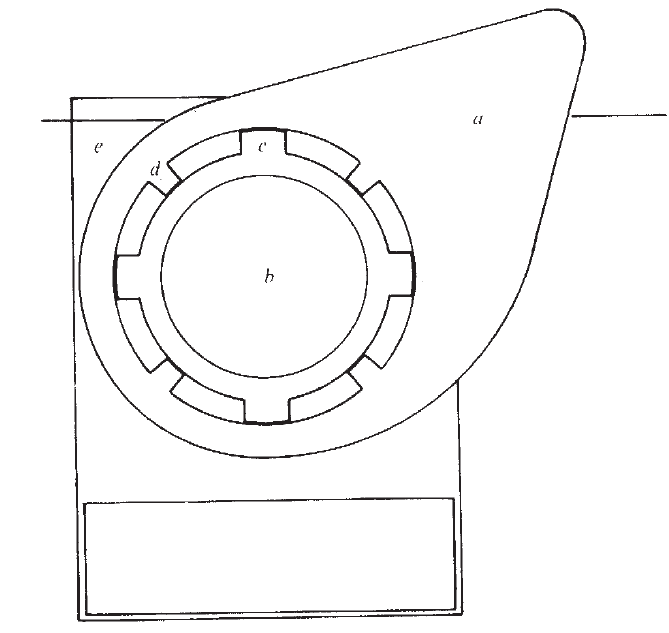
\includegraphics[scale=0.25]{graphics/duck}
\caption{A reproduction of a figure from ``Wave Power,''\cite{salterDuck}. ``a. vane; b, a hollow cylindrical member; c, paraxial ridges; d, inward facing ridges on the vane; e, vertical fin between this vane and the next.''}
\end{figure}

Salter is considered a foundational figure in the sector [REF]. By his own account in, ``Wave Power: Nostalgic Ramblings, future hopes, and heretical suggestions'' \cite{salterRamble} the early years of wave power are the history of him and his colleagues.

Salter received funding from the UK Department of Energy to set up a laboratory in Edinburgh. Wave power also garnered interest from other British academics, notably David Evans in Bristol who invented the Bristol Cylinder. (Evans, et al., 1979).
Evans also developed theories on the hydrodynamics and efficiency of WECs under idealised conditions (Evans, 1976). His work concerns a one-dimensional scenario where waves are modelled as perfect sinusoids that meet the WEC at right angles. This is not the case in nature and thus his claim that 100\% extraction of wave energy is possible has never been produced in practice.
Unfortunately, with the conclusion of the Oil Crisis, Salter and Evans found it increasingly difficult to secure funding for their research and none of their devices have been brought to market. In his Review article titled, ``Wave energy: Nostalgic Ramblings, future hopes and heretical suggestions,'' Salter blames pressure from the nuclear sector and ``others [who] set out to destroy what they saw to be a threat,'' (Salter, 2016). He then goes on to explain that whilst WECs were initially billed as very simple the reality is significantly more complex.
At the time of writing there have been two WEC projects in the UK that have reached commercialisation. Pelamis from Pelamis Wave Power and Oyster from Aquamarine Systems. (The European Marine Energy Center Ltd., 2019). Figure 2 shows these devices as they were installed. Pelamis 1 was installed in 2004 and became the first WEC to provide power to a National Grid. Pelamis 2 became the first WEC to be purchased by a utility company in 2009. Oyster was installed in 2012. Both devices provided power to the National Grid over the course of their lifetimes.

  
Figure 2: Pelamis 2 [Top] and Oyster [Bottom] as installed at the Billia Croo wave test site in Orkney, Scotland. (The European Marine Energy Center Ltd., 2019)
Similarly to Salter and Evans, both organisations found it difficult to secure funding after their initial funding lapsed. Both companies went into administration a few years after the installation of their WECs. This appears to be a recurring problem in the industry as there have been many other promising WEC projects that have failed to find investors. Examples include Corpower Ocean and Seatricity (The European Marine Energy Center Ltd., 2019).

It appears previous WECs were not economically viable as no WEC project to date has consistently made profit. Investors have also proven unreliable long-term. Barring global economic change there is a need to make WECs more profitable if they are to become a national power source.

One way of increasing the viability of a WEC is to use a control system. By taking the current Wave Excitation Force as an input the power extraction of a WEC can be optimised. In this project an in-development WEC known as WaveSub is used to investigate  the effectiveness of fixed gain control schemes for power optimisation.
The WaveSub device consists of a submerged cylindrical float tethered to an underwater platform via 4 cables. The cables drive Power Take Offs (PTOs) that can extract energy from the motion of the float relative to the platform. (Marine Power Systems, 2019)



Works from the 2019 EWTEC conference which use alternative tracking control do not exhibit this drift. The cause of the drift is unknown and represents a novel research subject. There has been comparatively little work on 6DOF WECs compared to planar devices like the Salter duck and Bristol Cylinder. This project will seek to replicate the drift result and will investigate its cause. Ideally the drift could be rectified without the need for additional control loops, retaining the computational simplicity of the scheme. Estimating the Wave Excitation Force becomes more complex in 6DOF. It is necessary to consider all the forces and Torques acting on the float. This can be represented as a 6×1 vector known as a Wrench, making it the Wave Excitation Wrench.

It may be possible to adapt existing work on Heave only WECs into this format. Nguyen and Tona have presented a detailed account on two methods of Wave Excitation Force estimation (Nguyen \& Tona, 2018). Alternately there is a wealth of research available on semi-analytical or computational methods. M. Folley’s book, “Numerical Modelling of Wave Energy Converters” (Folley, 2016) is a modern collection of these methods.

Finally, it is necessary to construct a state-vector for the system. In heave only WECs this is a single variable. For 6DOF WECs the state vector can be represented in the form of a 6×6 homogeneous matrix transform. There are two ways to derive this transform which are referred to as the active view and the passive view. (Merlet, 2006)
 The passive view has been successfully used in prior research (Hillis, et al., To Appear) however the active view may merit investigation. Since the WaveSub device is a class of cable robot its equations of motion can be derived using Screw Theory.
Given the forces on the float as a Wrench and its state as a Homogeneous Transform it is easy to write the equations of motion of the body. It is considerably harder to find solutions to the equations of motion since according to (Merlet, 2006) the space of all rigid body displacements in this or any equivalent system is non-linear (manifold).
Screw theory proposes to linearise these equations of motion by using the tangent space of all rigid body motions of the system. That is, by considering small displacements over small time periods a (virtual) velocity twist is constructed. The space of all velocity twists is linear.
Multiplying the velocity screw by the body’s inertia matrix (calculated from physical parameters) gives the momentum wrench. The equations of motion for the system can then be described as:

d/dt Momentum Wrench=Wave Excitation Wrench
This is now a non-linear first order differential equation which may be solved by numerical methods. Analytical solutions are usually impossible and certainly not practical for a digital controller.
J.P. Merlet’s book “Parallel Robots,” (Merlet, 2006) offers a comprehensive explanation of modelling cable robots, and J. Selig’s book, “Geometrical fundamentals of Robotics,” explains how to apply Screw Theory to parallel robots.

\chapter{Aims and Objectives}
The aims of this projected are phrased as 3 research questions.
\begin{enumerate}
\item{Does a drift problem occur if Ringwood's Simple and Effective Control strategy is adapted for planar motion?}
\item{If the drift problem exists, can it be resolved?}
\item{How much power does this implementation generate compared to an optimally tuned, passively damped system?}
\end{enumerate}

To answer these questions, it was necessary to achieve the following objectives.



\chapter{Research Methodology}
This research seeks to confirm the drift result previously produced by the project supervisor, Dr. Hillis. It makes use of much of his work as a foundation but seeks to reproduce his findings using independent work. By reviewing in this way it is hoped that a greater understanding of the Simple and Effective control method as it applies to multi-DOF WECs can be reached.

\section{Positivism and Simulation}
This research makes use of a positivist approach wherein hypotheses are proposed and then either refuted or not-refuted by physical evidence. This project is also a simulation-based project, and thus does not produce physical evidence.

This contradiction is resolved by the belief that a simulation can produce results that are indicative of results in the real world. To achieve this it is necessary to review all the assumptions and models that are used in the simulation. If the assumptions are flawed or the models inaccurate, then this belief is invalidated. 

In this scenario the author is both the creator of the system and of the test. It is possible to inadvertently bias results by including assumptions that increase the likelihood of significant results and excluding those that decrease the likelihood. To avoid this all simplifying assumptions will be catalogued. The results will be presented within the context of these assumptions.

Ideally simulations will be verified by real world tests. This does not usually occur unless a significant result has been found, and is therefore outside of the scope of this project. Until then self-examination must serve instead. If significant results are found then this project will serve as an inexpensive precursor to physical testing. If significant results are not found then physical testing may be applied more fruitfully elsewhere.

\section{Equipment}

\chapter{Simple and Effective Control}
Simple and effective control refers to a strategy presented by Fusco and Ringwood in their paper, ``A simple and effective real-time controller for wave energy converters,''\cite{ringwood}. This strategy was designed for a 1-DOF WEC, however the WaveSub device considered in this project is a 6-DOF device. This complicates the implementation of simple and effective control. Simplifying assumptions were made which are described in Section \ref{section: assumptions}. The most important of these is the assumption that the WaveSub device behaves as a planar device, and that only surge and heave motions are controlled. Therefore the control strategy need only be adapted for 2 DOF, rather than 6.

Figure \ref{fig:fullControl} shows the full implementation of the control strategy in the Simulink environment. This chapter will detail each component in sufficient detail that the reader may re-create the system. The input to the system is a 6 element vector of wave excitation forces in each dimension($F_{ex}$). The output is 6 element vector of float velocities in the same dimensions. The 6 dimensions and their order in the vector are Surge, Sway, Heave, Roll, Pitch, and Yaw.

\begin{figure}[b]
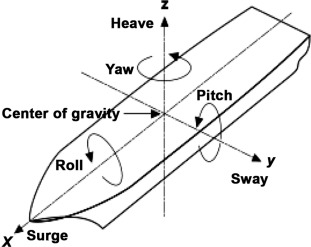
\includegraphics{graphics/dimensionsPic}
\centering
\label{dimensionsPic}
\caption{The 6 degrees of freedom relative to a boat. For the modelled float shown in figure \ref{fig:waveSub} the Yaw axis ($y$) is coincident with the cylindrical axis of the float. Figure reproduced from ``Deepwater Drilling''\cite{dimensionsPic}.}
\end{figure}

\begin{figure}[t]
\label{fig:fullControl}
\hspace{-2cm}
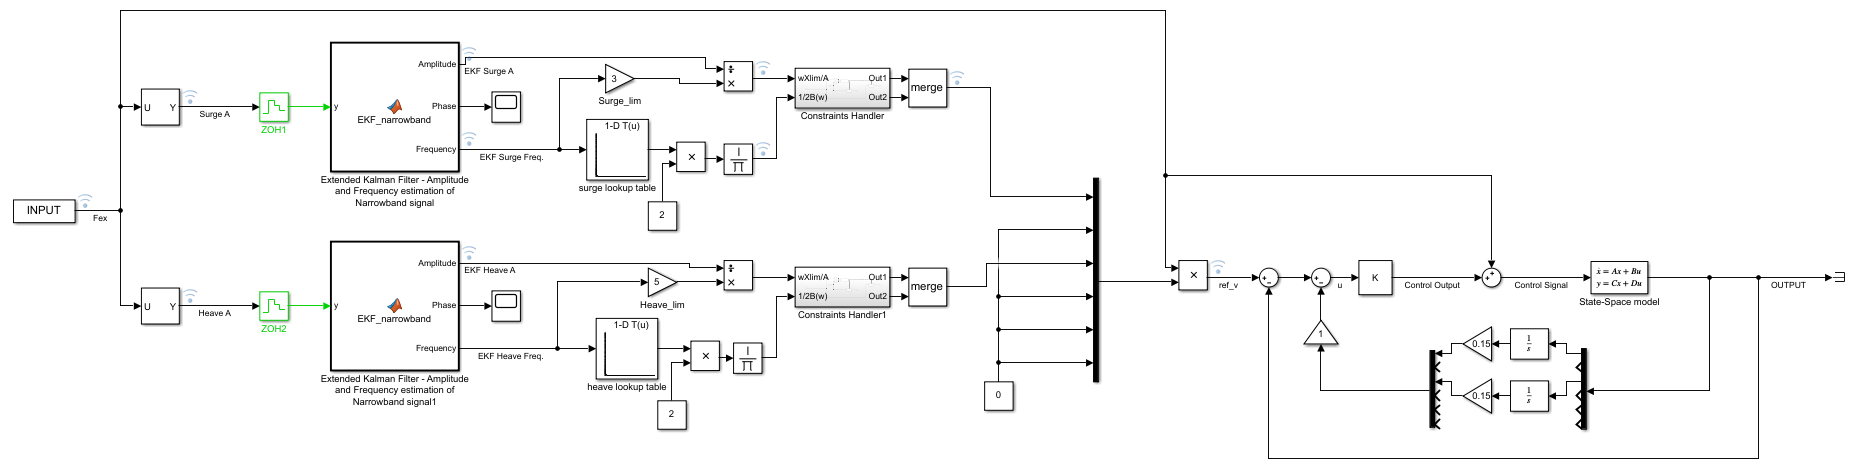
\includegraphics[scale=0.6]{graphics/fullControlSystem}
\caption{The full implementation of simple and Effective Control for the WaveSub device.}
\end{figure}

\FloatBarrier
%Fusco and Ringwood report that their control strategy provides, "levels of power capture close to MPC in most sea states... without the need of predictions and the solution of an optimization[sic] problem in real time."\cite{ringwood}. %Move this to another section.


\section{Simplifying assumptions}
\label{section:assumptions}

Sea states are modelled as irregular waves, meaning that they are the finite sum of many simple harmonic (regular) waves. Real life waves can be described perfectly as an infinite sum of regular waves, but this cannot be calculated in real-time. The waves are created from a random combination, rather than being based on recorded data.

The energy distribution within a generated irregular wave is modelled using an empirical relationship known as the Pierson-Moskowitz spectrum. The technique is fully described in "A proposed spectral form for fully developed wind seas based on the similarity theory of S. A. Kitaigorodskii," by Pierson and Moskowitz\cite{OGPM}. This spectrum relates wave frequency and energy distribution and is based on the assumption that sea waves are in equilibrium with the wind. A 2003 review paper using modern wave data reaffirmed that "for the chosen data only... [the spectrum] provides statistically robust relations."\cite{PMReview}

The float is modelled by a state-space model taken from the project supervisor's unpublished work\cite{andyMPC}. In this model it is assumed that the platform holding the PTOs is stationary. In the WECSim environment motion of the platform due to wave exctitation force is modelled.


\section{Internal Model Control}
Internal Model Control(IMC) involves creating a model of the plant, and then inverting it. The inverse model produces a  signal that will reproduce the control signal when given as input to the plant. This method is reliant on accurate modelling.

Figure \ref{fig:IMC} shows the implemented controller. It is a positive feedback loop, where the forward path is an inverse state-space model of the float, and the feedback path is the state space model. It is implemented as described in Ringwood's paper \cite{ringwood}.

\begin{figure}
\centering
\label{fig:IMC}
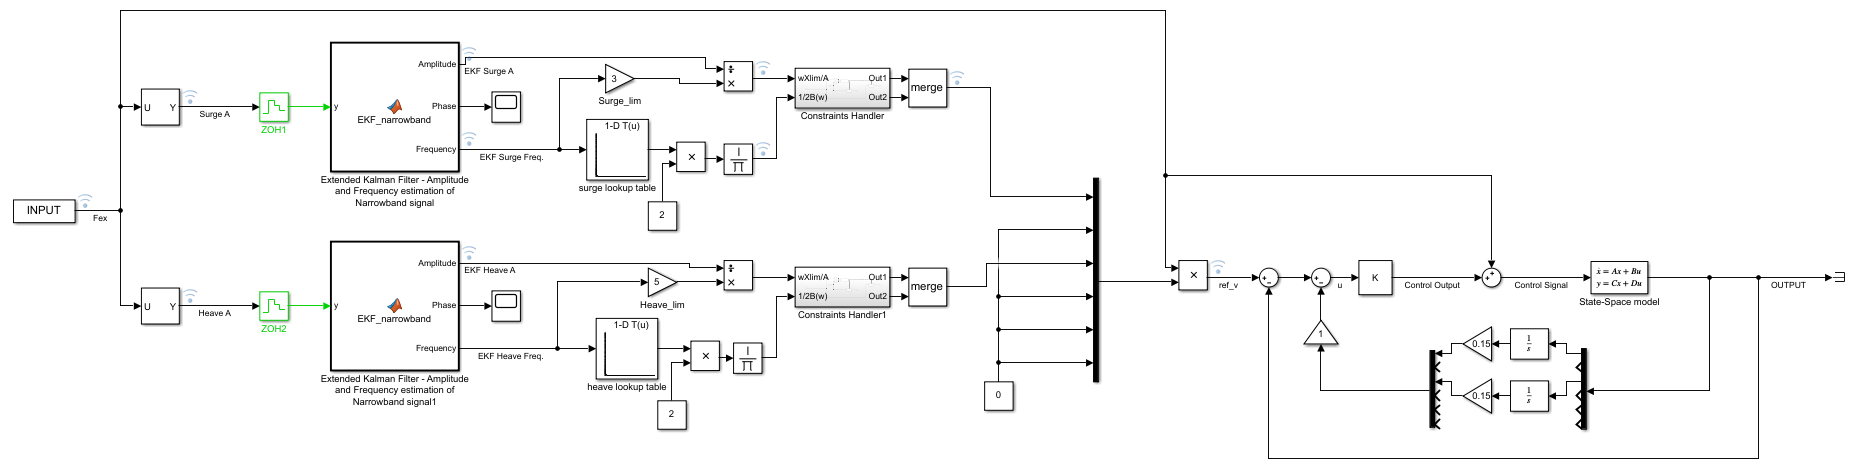
\includegraphics[scale=0.5]{graphics/fullControlSystem}
\caption{IMC implementation using an inverted state space model.}
\end{figure}

The model used is a state space model taken from unpublished work by the project supervisor \cite{andyMPC}. Its derivation is outside the scope of this project. It takes 3 input forces and 3 input torques, one for each DOF. It outputs 3 velocities and 3 angular velocities. The inversion of this state space model is novel work, and is detailed in section \ref{SSInverse} The only change is that the MATLAB command, "c2d" has been used to turn the continuous-time state-space model into discrete-time. Using discrete time also forces the Simulink Solver to use a known numerical method. This prevents errors cause by mismatched solver methods.

\section{Inverting the state-space model}
\label{SSInverse}
The desired inverse will map the outputs of the state-space model to its inputs.

One inversion method is to convert the state-space system into a system of transfer functions. In this case the inverse is the reciprocal of the transfer function. This method is complicated by the fact that the plant is a 6x6 MIMO system. Generating corresponding transfer functions using inbuilt MATLAB methods results in 36 high order transfer functions.

This over-fitting of the model can be corrected by manually fitting lower order transfer functions to the system. The project supervisor has used this approach in unpublished work\cite{AndyModelErrors}. The results of this work have been provided for comparison in the Results section.

Another inversion method known as the Massay-Sain algorithm has been used instead. It is able to overcome some of the shortcomings of the transfer function method. It does not require a filter to be stable; it calculates all cross terms; and does not over-fit the model.

The Massey-Sain algorithm was first presented by Sain and Massay in 1969\cite{OGMassaySain}. In 2004 it was summarised in a lecture given by Professor S. Sundaram\cite{Sundaram}. The following derivation is paraphrased from Sundaram's lecture and simplified.

First it is necessary to test whether or not the system is invertible. All discrete-time state space systems are of the form
\begin{equation}
\label{definition1}
	x(t+1)=Ax(t)+Bu(t)
\end{equation}
\begin{equation}
\label{definition2}
	y(t)=Cx(t)+Du(t)
\end{equation}

Where $x$ is the state vector; $y$ is the output vector; $u$ is the input vector; $A$ is the state matrix; $B$ is the input matrix; $C$ is the output matrix; and $D$ is the disturbance matrix.

For our system there is no disturbance input and so $D$ is the zero matrix. It will not be shown in further equations.

From Sundaram,
"A system has an inverse with delay $L$ if $u(t)$ can be uniquely determined from $y(t),y(t+1),…y(t+L)$  (and perhaps $x(t)$)."\cite{Sundaram} So values of $L$ must be tested to see if $u(t)$ can be uniquely determined.

It is possible to express later time-steps in terms of the current time step via substitution.
\[					%delimiters for 'displaymath' environment, no numbering.
	y(t+1)=Cx(t+1)
\]

Substituting equation \ref{definition1},
\[
	y(t+1)= Ax(t)+Bu(t)
\]

This can be iterated for any number of time steps. It can also be represented in a matrix format:

\[
	\begin{bmatrix}
		y(t)   \\
		y(t+1) \\
		y(t+2) \\
		\vdots \\
		y(t+L)
	\end{bmatrix}
	=
	\begin{bmatrix}
		C   \\
		CA  \\
		CA^2\\
		\vdots\\
		CA^L
	\end{bmatrix}
	x(t) +
	\left[
	\begin{array}{c|cccc}			%Have to use 'array' to do partitions
	0&0&0&\hdots&0						\\
	CB&0&0&\hdots&0						\\
	CAB&CB&0&\hdots&0					\\
	\vdots&\vdots&\vdots&\ddots&\vdots	\\
	CA^{L-1}B & CA^{L-2}B & CA^{L-3}B & \hdots & 0
	\end{array}
	\right]
	\left[
	\begin{array}{c}
		u(t)		\\
		\hline
		u(t+1)		\\
		u(t+2)		\\
		\vdots		\\
		u(t+L)
	\end{array}
	\right]
\]
\begin{equation}
\label{LTimesteps}
=Y_{(t,L)} = O_Lx(t)+M_L U_{(t,L)}
\end{equation}

Where $O_L$ is analogous to the Observability of the system, and $M_L$ to its Measurability. The partitions show that $M_L$ contains the smaller matrix $M_{L-1}$. This can be iterated for all versions of $M_L$ down to $M_0$.

Massey and Sain's theorem\cite{OGMassaySain} asserts that if the rank of $M_L$ minus the rank of $M_{L-1}$ is equal to the number of columns $'m'$ of $M_{L-1}$ then there exists a matrix $\mathcal{K}$ such that
\[
\mathcal{K}M_L =
\left[
\begin{array}{c|c}
I_m & 0
\end{array}
\right]
\]
Multiplying equation \ref{LTimesteps} by $\mathcal{K}$,
\[
\mathcal{K}Y_{t,L} = \mathcal{K}O_Lx(t) + u(t)
\]
Hence the input $u(t)$ can be expressed in terms of the outputs $Y_{t,L}$

\begin{equation}
\label{inverseDefinition1}
u(t) = -\mathcal{K}O_Lx(t) + \mathcal{K}Y_{t,L}
\end{equation}

Similarly the state vector at time $t+1$ can be found by substituting equation \ref{inverseDefinition1} into equation \ref{definition1},
\begin{equation}
\label{inverseDefinition2}
x(t+1) = (A-B\mathcal{K}O_L)x(t) + B\mathcal{K}Y_{t,L}
\end{equation}

Equations \ref{inverseDefinition1} and \ref{inverseDefinition2} together represent the inverse State-space model.

The task is now to see if there exists a value of L for our system that will satisfy the Massey-Sain theorem. In the case that there are multiple viable values of L the smallest value is preferable as any inverse constructed with it will have the smallest possible delay.

In the case of our 6 input, 6 output system $M_0$ is the $6\times6$ zero matrix. It has rank 0, and 6 columns($m=6$).

$M_1$ has the form
\[
\left[
\begin{array}{cc}
0	&	0	\\
CB	&	0	\\
\end{array}
\right]
\]
where $CB$ is a full-rank $6\times6$ matrix, making the overall rank 6.

Therefore the system is invertible with $L=1$ since
\[
rank(M_1) - rank(M_0) = m_0
\]

As above the matrix $\mathcal{K}$ is formed by performing a pseudo-inverse of $M_1$ less the last 6 columns. This is done using the pinv() command in MATLAB. This results in a $12\times6$ matrix. This is expected since
\[
Y_{t,L} = Y_{t,1} =
\begin{bmatrix}
y(t)	\\
y(t+1)
\end{bmatrix}
\]

To find the inverse at the time-step $t+1$ the inverse system must be given both $y(t)$ and $y(t+1)$. since y is a $6\times1$ vector this makes $Y_{t,1}$ a $12\times1$ vector which matches the dimensions of $\mathcal{K}$.

The inverse can then be constructed in Simulink, according to equations \ref{inverseDefinition1} and \ref{inverseDefinition2}, using the discrete state-space block. A one time-step delay is needed to generate $y(t)$ at the timestep $t+1$. This is shown in Figure\ref{fig:inverseSS}.

\begin{figure}
\centering
\label{fig:inverseSS}
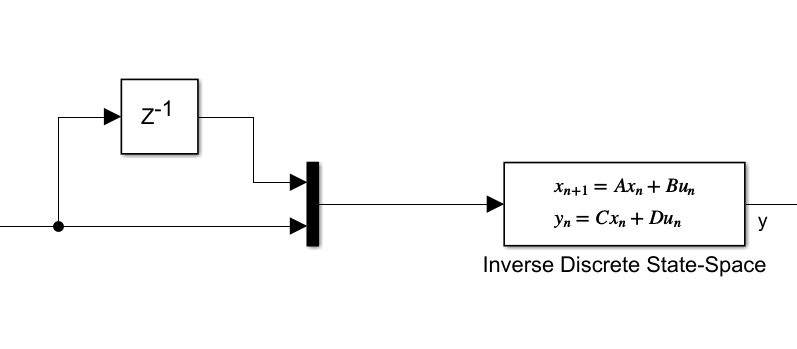
\includegraphics[scale=0.5]{graphics/inverseSS}
\caption{The inverted state space model with the a one time-step input delay.}
\end{figure}

This results in a robust inverse system. When used in the IMC loop it is able to perfectly track simple sinusoid input at a one time-step delay. This delay is negligible for sufficiently small time-steps.

\section{Adaptive law}
\label{adaptiveLawSection}
%Figure of Ringwood's Control system somewhere?
Ringwood's paper\cite{ringwood} on Simple and Effective control makes use of an adaptive filter described as 
$\frac{1}{H(t)}$.  This filter takes the dominant frequency and amplitude of the incoming wave excitation force($F_{ex}$) and outputs a reference velocity($v_{ref}$). The control system then makes the float track this reference velocity as accurately as possible.

Ringwood has shown through extensive study that maximum energy extraction in 1DOF occurs when the float oscillation is in phase with the excitation force's dominant frequency\cite{ringwood}. So to realise maximum energy extraction, ``The velocity should always be in phase with the excitation force and it should have an amplitude that is modulated in the frequency-domain by the inverse of double the radiation resistance $\frac{1}{2B(\omega)}$''\cite{ringwood}.

This is expanded to cover the two controlled dimensions of the float: Surge and Heave. It is assumed that maximum power extraction may be achieved in both dimensions as they are independent. For example, uneven excitation in these two dimensions will result in elliptical motion of the float.

To construct the filter the radiation response of the float in each dimension must be modelled. The radiation response refers to the forces on the float due to the waves that are generated by the float's motion, and which then carry energy away from the system. These responses can be modelled by transfer functions. The project supervisor has provided these transfer functions and they are shown in appendix \ref{radiationTFs}.

These functions transfer float velocity to radiation force. We need to find the amplitude of the radiation response at a given frequency. Bode plots relate the amplitudes and frequencies of systems. Figure \ref{bodePlots} shows bode plots of both functions.

\begin{figure}
\label{bodePlots}
\caption{Bode plots of the Surge and Heave radiation force transfer functions. Created using the Simulink bode plot block.}
\end{figure} 

The data from these plots is then turned into lookup tables to be used in the filter as shown in the code in appendix \ref{inputFile}. Now given the dominant frequency of $F_{ex}$ the radiation amplitude response can be obtained using the lookup table block in Simulink as shown in figure \ref{fig:adaptiveLawsimulink}. According to Ringwood\cite{ringwood} the velocity reference may be obtained via the relation,

\[
v_{ref}(t)=\frac{1}{2B(\hat{\omega})}f_{ex}(t)
\]

where $\hat{\omega}$ is the radiation force amplitude response produced by the dominant frequency. This is implemented as shown in figure \ref{adaptiveLawSimulink}. Hence $v_{ref}$ is obtained and given as an output.
 
\begin{figure}
\label{adaptiveLawSimulink}
\caption{The fully implemented adaptive filter in the Simulink environment.}
\end{figure} 


\section{Filtering Wave Excitation Force}
\label{EKF}
It is necessary to make an estimate of the frequency of $F_{ex}$ in order to produce $v_{ref}$ as described in section 
\ref{adaptiveLawSection}. A kalman filter is used to extract these parameters from $F_{ex}$. The programming of the kalman filter block was provided by the project supervisor, and the tuning of it was performed by the author.

Kalman filters are commonly used 

\begin{figure}
\label{kalmanAmplitudeEnvelope}
\caption{}
\end{figure} 

\begin{figure}
\label{kalmanFrequency}
\caption{}
\end{figure} 


\section{Constraints Handling}
\label{constraintsHandlingSection}
The control strategy has so far only focused on tracking the best velocity for energy capture. There are also physical constraints which must be considered. Motions in all of the non-controlled dimensions are already very small and  need not be specifically controlled. In the controlled dimensions of heave and surge there are large amplitude motions which may exceed the physical limits of the device.

For the WaveSub device the physical limits in heave and surge are $\pm 5m$ from the home position. A limit of $\pm 3m$ is imposed in the surge dimension as a safety factor and for improved performance. It is important that the float does not crash into the platform.

Ringwood \cite{ringwood} proposes a method to limit the amplitude of the velocity, which prevents the float from deviating outside of physical limits so long as the mean of the float's velocity is zero. As shown in the results in chapter \ref{results} this is not necessarily the case.

To impose this limit a new term is calculated which can be expressed as, 

\[
\frac{\hat{\omega}X_{lim}}{\hat{A}}
\]

where $\hat{\omega}$ is the frequency of $F_{ex}$; $\hat{A}$ is the amplitude of $F_{ex}$ in metres; and $X_{lim}$ is the physical limit in the relevant dimension in metres.

The adaptive law from section \ref{adaptiveLawSection} is then modified with conditional logic such that,

\[
\frac{1}{H(t)} = 
\left\{\begin{matrix*}[l]
\frac{1}{2B(\hat{\omega}}, \textup{ if } \frac{\hat{\omega}X_{lim}}{\hat{A}}>\frac{1}{2B(\hat{\omega})}\\
\frac{\hat{\omega}X_{lim}}{\hat{A}}, \textup{ otherwise.}\\
\end{matrix*}\right.
\]

Figure \ref{velocityConstraints} shows how this logic was implemented in Simulink.

\begin{figure}
\label{velocityConstraints}
\caption{}
\end{figure}


\section{Integral feedback}

Implementation of the prior sections of this chapter is all that is needed to fully realise Ringwood's Simple and Effective control. However, as shown in the results in chapter \ref{results} this results in a drift that quickly violates physical constraints. This drift may arise due to the fact that the mean of the float's velocity is non-zero. This would mean that limiting the amplitude of the velocity as described in section \ref{constraintsHandlingSection} is insufficient.

Introducing an integral feedback loop may resolve this issue. There are many ways to implement this. Figure \ref{integralFeedbackLoop} shows one. There are two summing junctions in the figure. Routing the integral feedback path to either one produces a different implementation. 

\begin{figure}
\label{integralFeedbackLoop}
\caption{}
\end{figure}

In this project it was found that the implementation as shown in figure \ref{integralFeedbackLoop} produced better power results and better managed the physical constraints. See chapter \ref{results} for details.

The gain was tuned with the constraints turned off. It keeps the mean of the velocity to within $0.1ms^{-1}$ of 0. Ringwood's constraints can then be used to limit the velocity, and therefore the position, as intended.

\chapter{Results}
\label{results}

All simulations presented here have been created using wave data generated by WecSim according to the Pierson-Moskowitz spectrum relation \cite{OGPM} with a sampling rate of $\frac{1}{0.02s}=50Hz$.


\section{Difficulties with the WecSim environment}
Despite the author's best efforts the control system could not be realised in the WecSim environment within the project time frame. In every implementation the float's response was unstable, and physical constraints were violated within 10 seconds. Figure \ref{wecsimUnstable} shows a typical, unstable, result. The WecSim environment is unable to produce meaningful results once kinematic constraints have failed, and instead throws an error then shuts down. This has prevented the collection of meaningful results.

\begin{figure}
\label{wecsimUnstable}
\caption{A plot of Velocity over time of the float as simulated in WecSim. Only the first few seconds are available as the system is unstable and violates physical constraints quickly.}
\end{figure} 

The model produced by Dr. Hillis was able to run in the author's instance of WecSim. This implies that the issue lies in the control system produced by this project, or in some interaction between the WecSim environment and the control system that is not present for the other system.

There are many potential causes of the instability. At the time of writing the issue remains unsolved, so all causes listed here are merely speculation. Further work is needed to determine the true cause. 

Some model mismatch exists between the state-space model and the WecSim model. It was assumed that this mismatch was insignificant as detailed in section \ref{section:assumptions}. This may be mistaken.

The developed control system features a real-time delay where Dr. Hillis' system does not. When transforming to the frequency domain a real-time delay becomes an exponential term. For example, if a function $f(t)$ is shifted by time $a$,
\[
\mathcal{L}[u(t-a)f(t-a)]=e^{-as}F(s)
\]
This exponential term could be responsible for the instability.

Finally there may be a bug or unconsidered effect in the WecSim source code that produces this instability for the developed control system but not for Dr. Hillis' system.

In place of the WecSim environment, the state-space model used for development of the IMC was used to produce results. This is undesirable since it makes more assumptions than the WecSim environment, and it was the basis of the control system's development. By using the model from which the control system was derived, modelling error is completely eliminated. This means that no evidence can be produced on the system's robustness against model errors.

\section{Tracking Performance}
The tracking performance is ideal save for a delay of one time-step due to the use of the state-space model as the plant. Figure ? shows a typical example of this tracking of reference velocity.


\section{Power Comparison}
(say that more red = more power)

The power generated by the system is compared against the power generated by an optimally tuned passively damped system as described in ``Active control for multi-degree-of-freedom wave energy converters with load limiting'' \cite{AndyMPC}.

This passive-damping system relies only on a damping co-efficient that relates cable velocity to cable tension. i.e.,

\[
Cable Tension = Cable Velcoity \times Damping Co-efficient
\]

in the axis of each cable. The co-efficient C is optimally chosen for each wave period. This could feasibly be performed in reality using an adaptive law and a method of measuring the sea-wave frequency such as the EKF method described in section \ref{EKF}.

Table \ref{passiveResults} shows the power generated in each sea state by the passively damped system.

\begin{table}
\label{passiveResults}
\hspace{-3cm}
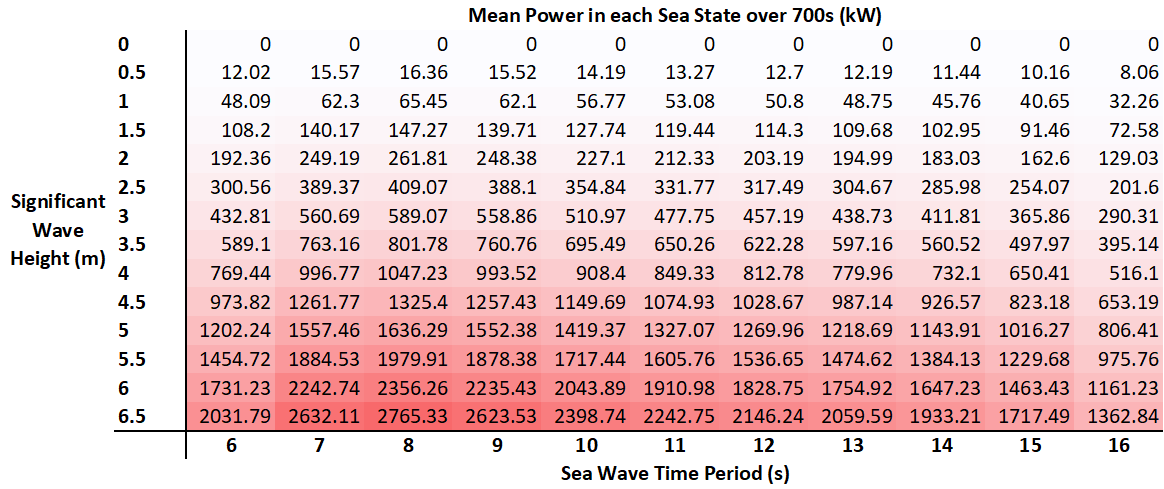
\includegraphics[scale=0.7]{tables/passiveResults}
\caption{Power generated by optimally tuned passive damping. Reproduced from\cite{andyMPC}.}
\end{table}

\begin{table}
\hspace{-3cm}
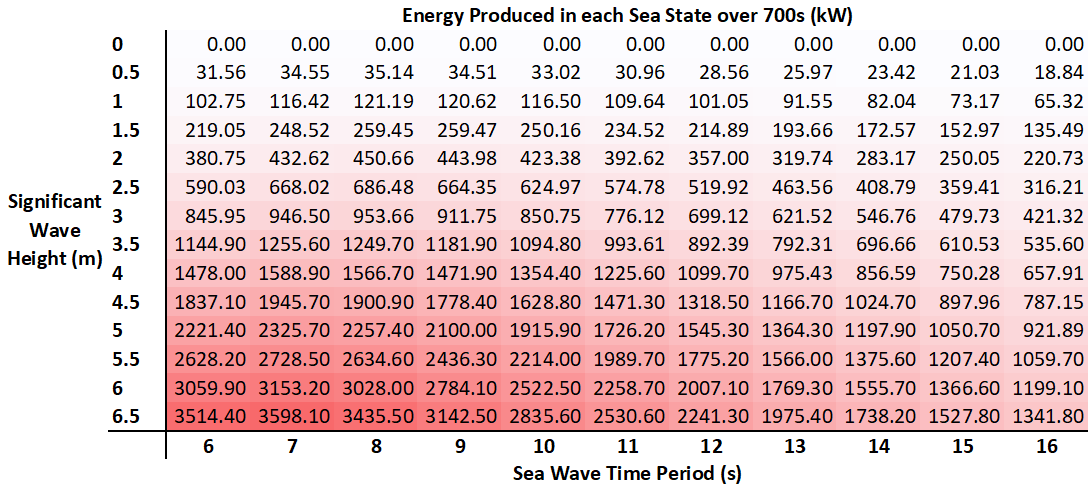
\includegraphics[scale=0.7]{tables/integralControlResults}
\caption{Power generated by integral feedback model. Darker red indicates higher power.}
\end{table}

\begin{table}
\hspace{-3cm}
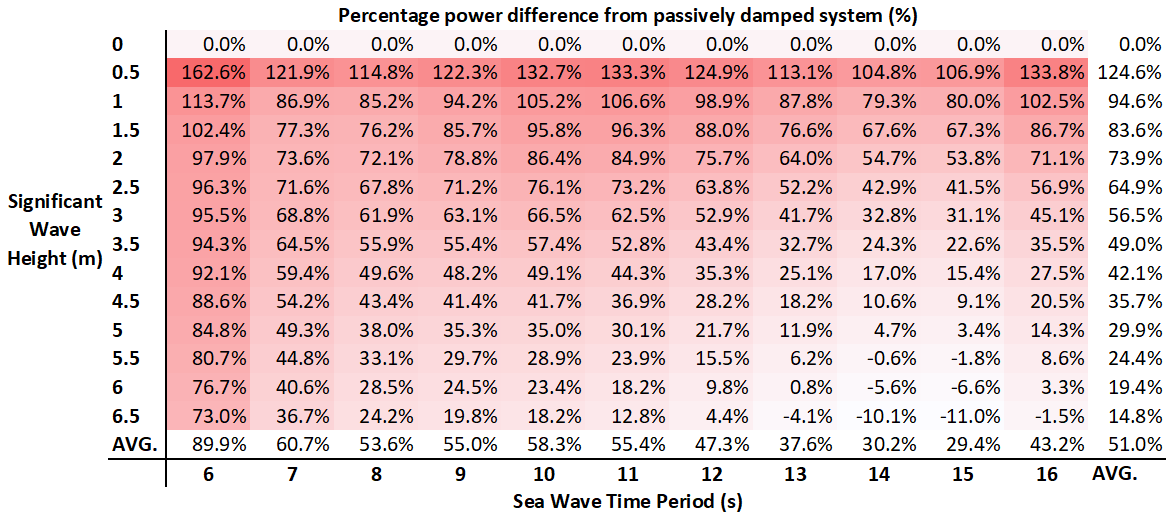
\includegraphics[scale=0.7]{tables/integralControlPercent}
\caption{Power generated by integral Positional control.}
\end{table}

\chapter{Discussion}
-Massay Sain is a robust inverse with high amp response at low frequency.
-Strong evidence drift problem exists.
	-Suspect Ringwood position constraints are flawed for real-world application. Non-zero mean. (Do a bit of maths?)
-Weak evidence of good power generation
-Integral Position constraints sorta work

\chapter{Conclusions}
In this work [something] has been done.

Answer to Q1: Drift problem exists. (non-zero mean)
Answer to Q2: Problem can be adressed using a variety of methods. Integral positional control shown to work.
Answer to Q3: Better power generation achieved (except for violent sea states). Further improvement possible. See results for exact figures.

In addition Massay-Sain inverse method introduced.

Looked at novel integral feedback loop. Empirical result - not supported by theory.

Hope that this contributes to the field.

\section{Future Work}

Any future work using the Massay-Sain inverse method in this field should investigate its robustness against model error.

Need to get working in WecSim.

Determine whether power increase can be obtained by adaptive law on integral Velocity control.


%\begin{sidewaysfigure}[h]
%	\centering
%	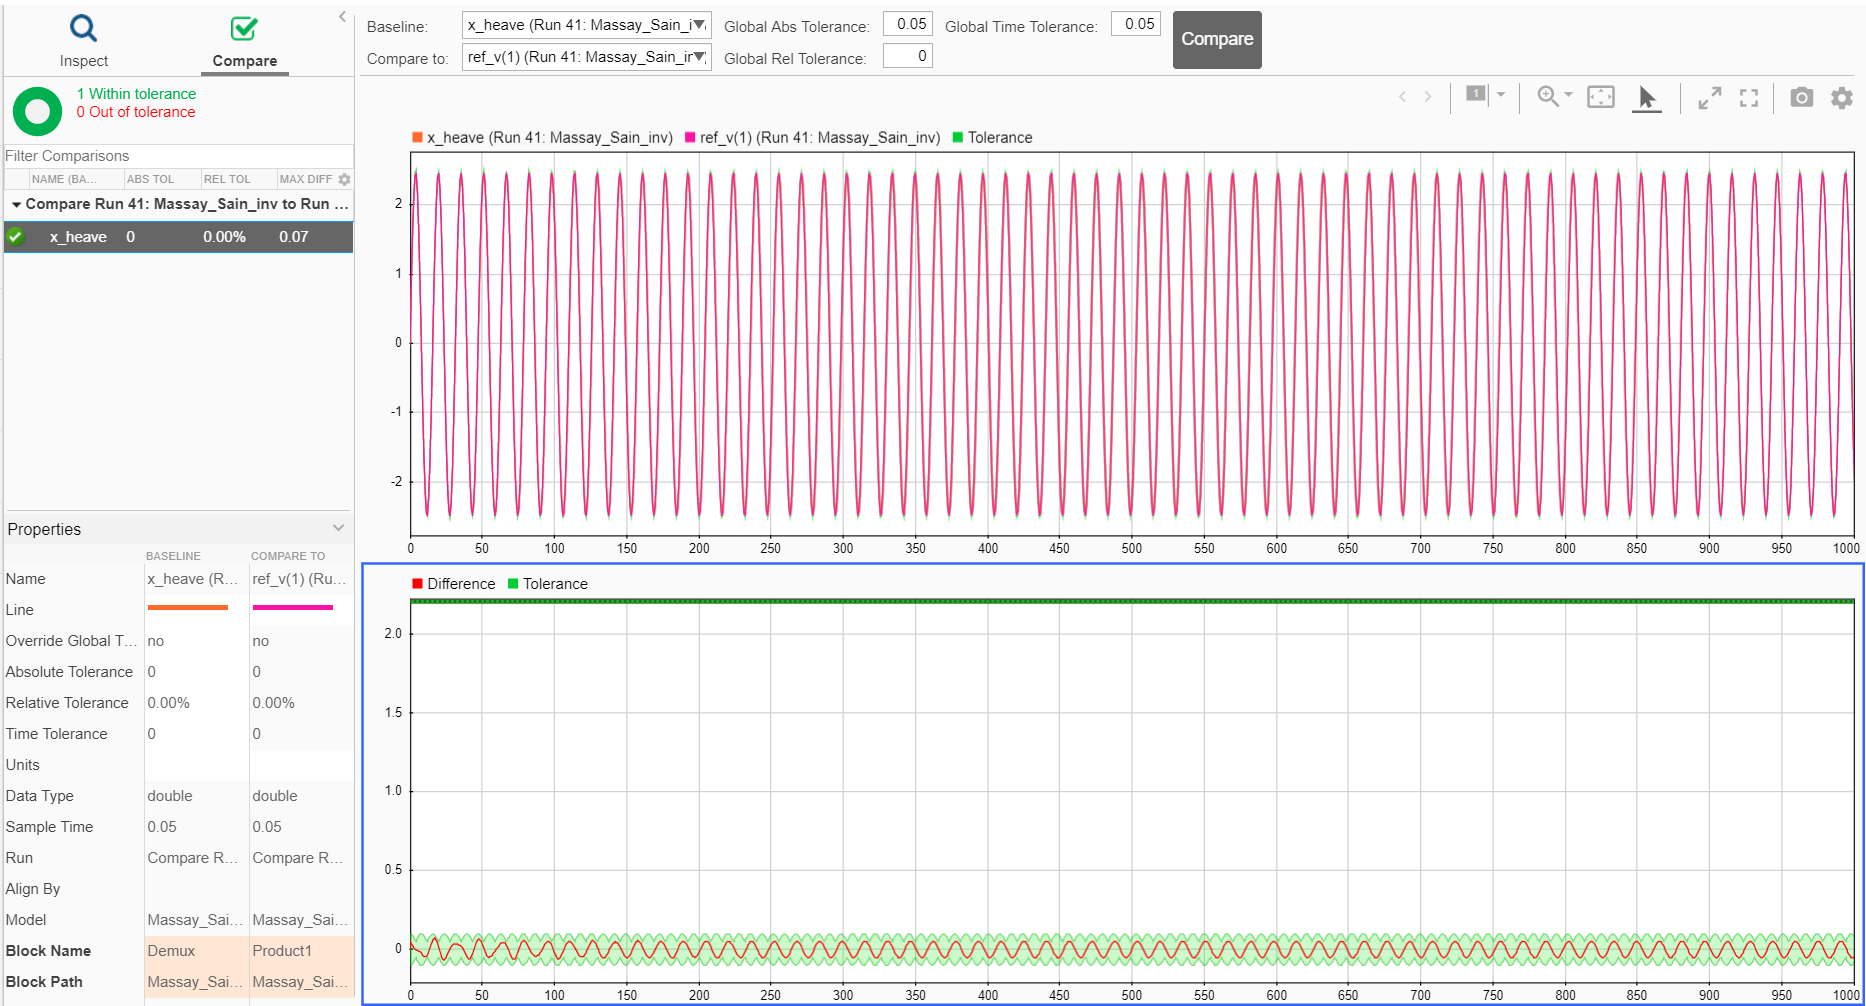
\includegraphics[scale=0.55]{heaveTracking}
%	\caption{A simulink data inspector comparison of the heave input and the output of the control loop. The input was a sinusoid with amplitude $10^6m$ and frequency $0.4rads^{-1}$. The time step was $0.05s$. The output matches the input with a global tolerance of $0.05 units$.}
%\end{sidewaysfigure}

\bibliography{bibliography}
\bibliographystyle{IEEEtran}

\appendix
\appendixpage
\addappheadtotoc
\chapter{Radiation force Transfer Functions}
\label{radiationTFs}

\chapter{Project code: inputFile.m}
\label{inputFile}

\end{document}